\documentclass[a4paper,14pt]{extarticle}
\usepackage[utf8]{inputenc}
\usepackage[english,russian]{babel}
\usepackage{amsmath,amsfonts,amsthm, mathtools}
\usepackage{amssymb}
\usepackage{graphicx}
\graphicspath{{images/}}
\usepackage{wrapfig}
\usepackage{floatrow}
\usepackage{setspace}
\usepackage[margin=10pt,font={small,stretch=0.9},labelfont=bf,labelsep=period,
justification=centerlast]{caption}
\usepackage{array,tabularx,tabulary,booktabs}
\RequirePackage{multirow}
\RequirePackage{multicol}
\RequirePackage{longtable}
\usepackage{indentfirst}
\usepackage{hyperref}
\usepackage{icomma}
\newcommand*{\hm}[1]{#1\nobreak\discretionary{}
	{\hbox{$\mathsurround=0pt #1$}}{}}
\usepackage{soulutf8} 
\usepackage{etoolbox} 
\usepackage{fancyhdr}
\renewcommand{\headrulewidth}{0mm} 
\cfoot{\thepage} 
\usepackage{geometry}
\geometry{top=20mm}
\geometry{bottom=20mm}
\geometry{left=20mm}
\geometry{right=20mm}
\DeclareMathOperator{\sgn}{\mathop{sgn}}

\begin{document}
		\begin{titlepage}
			\begin{center}
				\large Московский физико-технический институт\\
				(национальный исследовательский университет)\\
				\vspace{1cm}
				\begin{figure}[h!]
					\centering
					
\includegraphics[width=0.7\linewidth]{MIPT.jpeg}
					\label{fig:mpr}
				\end{figure}
				\vspace{4cm}
				\textbf {Название потом придумаю}\\
			\end{center}
			
			\vspace{9cm}
			{\par \raggedleft \large Выполнил:\\ студент 1 курса ЛФИ \\ Сливка Глеб \par}
		\end{titlepage}
		\tableofcontents
		\newpage
		\section{Теоретические сведения}
		
		\subsection{Необходимы определения машинного обучения}
		\textbf{\underline{Опр.}} \textit{Гиперпараметр} --- параметр машинного обучения, значение которого используется для управления процессом обучения. Его значение устанавливается перед началом обучения, в отличие от значений других параметров (обычно весов узлов), которые определяются во время обучения.
		
		\textbf{\underline{Опр.}} \textit{Операция оценки функции} --- это процесс определения, насколько хорошо модель машинного обучения способна предсказывать значения целевой переменной на основе входных данных.
		
		Оценка функции производится путём сравнения предсказанных значений модели с фактическими значениями целевой переменной. Чем ближе предсказания модели к фактическим значениям, тем выше оценка функции и тем лучше модель способна выполнять предсказания.
		
		\textbf{\underline{Опр.}} \textit{Функция стоимости}  --- это функция, которая измеряет стоимость или ошибку модели в зависимости от ее параметров. Она используется для оптимизации модели путем настройки ее параметров таким образом, чтобы минимизировать стоимость или ошибку.
		
		
		\textbf{\underline{Опр.}} \textit{Функция потерь} --- это функция, которая измеряет разницу между предсказанными значениями модели и фактическими значениями целевой переменной. Она используется для оценки качества модели и настройки ее параметров.
		
		Функция потерь определяет, насколько хорошо модель выполняет задачу, которую она должна решать. Чем меньше значение функции потерь, тем лучше модель соответствует данным и делает более точные предсказания.
		
		\textbf{\underline{Опр.}} \textit{Байесовская оптимизация} --- это метод оптимизации функций, который использует байесовский подход для поиска оптимальных значений гиперпараметров модели.
		
		В машинном обучении, модель может иметь гиперпараметры, которые не могут быть обучены напрямую из данных, и требуется выбрать оптимальные значения для этих гиперпараметров. Байесовская оптимизация позволяет находить оптимальные значения гиперпараметров, минимизируя количество итераций обучения модели.
		
		
		То есть байесовская оптимизация находит такое $x' \in \mathbb{R}^n$ --- набор неизвестных гиперпараметров на данном множестве $X$, что функция $f$ принимает максимальное значение: 
		$$ x' = \underset{x \in X}{argmax}[f(x)]. $$

		На каждой итерации алгоритм может вычислить оптимальный $x$ и сверить его с реальным тем самым можно \textit{производить операцию оценку функции}. 
		
		\subsection{Гауссовский процесс}
		Рассмотри индекс $x' \in \mathbb{R}^n$ и гауссовский процесс $f(x)$. Определим функцию среднего
		
		$$ m(x) = \mathbb{M} f(x),$$
		которая показывает среднее значение функции, и функцию ковариации
		
		$$ k(x, x') =  \mathbb{M}[(f(x)-m(x))(f(x')-m(x'))],$$
		которая показывает как изменение одной переменной связано с изменением другой переменной.
		
		\textbf{\underline{Опр.}}  $f(x)$ --- \textit{Гауссовский процесс (ГП)} , если $\forall n \in \mathbb{N}$ и $\forall x_1, x_2, \ldots, x_n$ величина $X = (f(x_1), \ldots, f(x_n))$ имеет многомерное гауссого распределение с вектором среднего $\mathbb{M} x = (m(x_i))_{i=1}^n$ и матрицей ковариации $\mathbb{D}x=(k(x_i, x_j))_{i, j}$. 
		
		Мы будем работать со стационарными ГП, поэтому $m(x) = const$. Если положить $m(x) = 0$, то ничего в задаче не поменяется. 
		
		Самый распространённый выбор функции корреляции (ядра ГП) --- экспоненциальное ядро: 
		
		$$ k(x, x') = \alpha^2  \cdot \exp\left[-\frac{1}{2 \lambda} (x-x')^T(x-x')\right],$$

		где $\alpha$, $\lambda$ --- гиперпараметры ядра.
		
		\subsection{Задача нелинейной регрессии}
		Пусть мы знаем значение функции $f$ в точках $x_1, x_2,  \ldots, x_n$ и \\ $(f(x_1), f(x_2), \ldots, f(x_n)) =  (f_1, f_2, \ldots, f_n) = f$. Задача нелинейной регрессии сводится к поиску значению функции $f$ в произвольной фиксированной точке $x'$. 
		
		Так как $f(x')$ ---  случайная величина, то плотность вероятности по формуле Байеса вычисляется следующим образом: 
		
		$$ p(f(x') | f_1, \ldots, f_n) = \frac{p(f(x'), f_1, \ldots, f_n)}{p(f_1, \ldots, f_n)} = {\mathcal {N}}(f(x) | \mu ,\sigma ^{2}).$$

		Мы получили нормальное распределение. Определим матрицу $K$:
		
		$$K = \begin{pmatrix} C & k \\ k^T & k(0)\end{pmatrix},$$
		где 
		
		$$C = (k(x_i, x_j))_{i, j = 1}^n, \; \; \; k_i = k(x_i, x').$$
		 Тогда математическое ожидание и дисперсия записываются в следующем виде: 
		 
		 $$\mu = k^TC^{-1}f,$$	
		 $$ \sigma^2 = k(0) - k^TC^{-1}k.$$
		 Используя эти формулу можно найти распределение функции в каждой новой точке. 
		 
		Пусть у нас есть выборка из четырёх точек, тогда $\nu$ будет проходить через все эти точки, и $\sigma^2$ будет определять доверительный диапазон. На рисунке ниже показано, как будет менять функция при добавление новых точек в выборку. 
		\begin{figure}[H]
			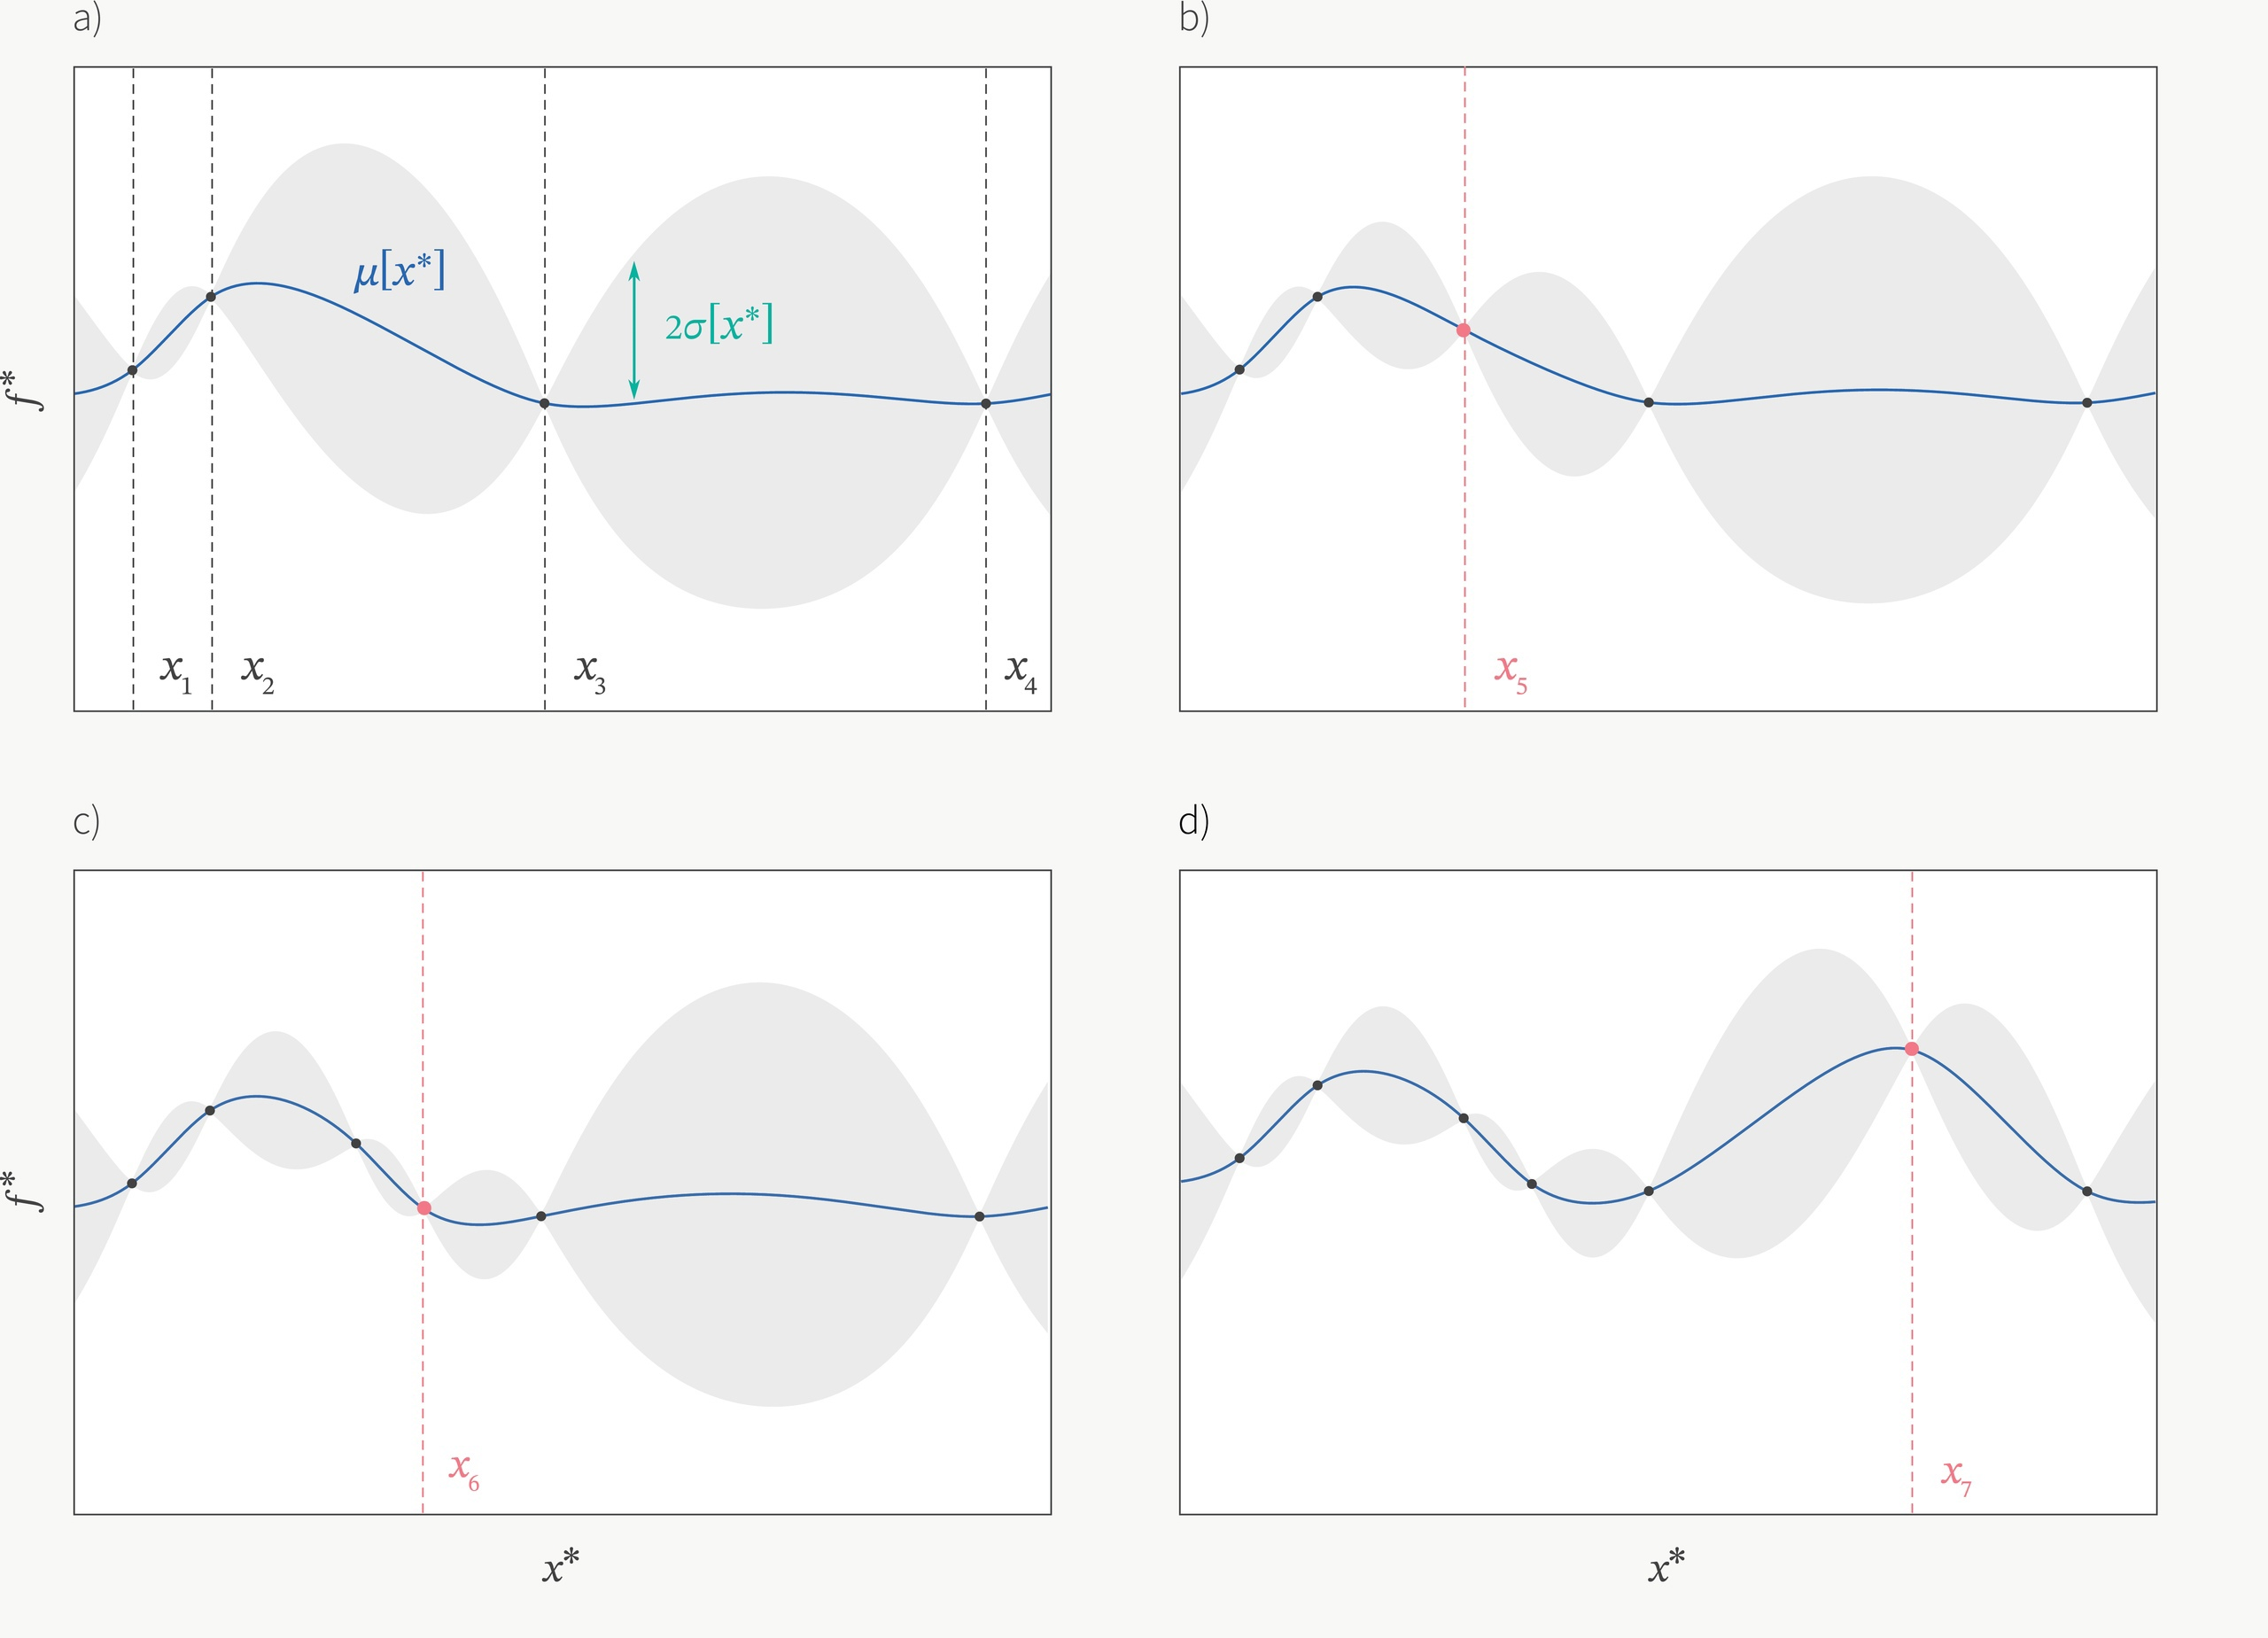
\includegraphics[scale=0.15]{p1}
		\end{figure}
	
		Также стоит отметить, что если $x'$ --- точка далёкая от точек выборки, то есть $k(x, x') \rightarrow 0$, тогда вектор $k \rightarrow 0$, значит функция стремится к 0. То есть, если мы обладаем конечной выборкой, то на бесконечности функция будет стремится к 0. 
		
		Так как на бесконечности $k \rightarrow 0$, то 	$\sigma^2 \rightarrow k(0)$, то есть доверительный интервал будет конечным и постоянным. 
		
		\subsection{Оптимизация}
		Пусть у нас есть выборка $y(x_1), \ldots, y(x_n)$ для оптимизируем функции. Решим задачу регрессии с помощью гауссовского процесса и получим некоторую функцию $f(x)$. Чтобы оценить,  насколько полезно будет исследовать конкретную точку в пространстве параметров вводят Acquisition функцию. Она основывается на текущей модели целевой функции и может учитывать различные факторы, такие как неопределённость модели (например, доверительный интервал), предполагаемое улучшение (например, насколько сильно значение целевой функции может быть улучшено в данной точке) и баланс между исследованием и использованием уже известной информации. 
		
		Acquistion функции принимают среднее и дисперсию в каждой точке x функции и вычисляют значение, которое описывает насколько желательно выбирать эту точку в следующий раз. 
		
		Модно придумать много разных Acquistion функций, мы рассмотрим следующую функцию: 
		
		$$f_{AC}(\theta) = \alpha\mu(\theta) + \beta \mu(\theta),$$
		
		где $\mu(\theta)$ --- значение, предсказанное ГП в точке $\theta$ со стандартным отклонением $\sigma(\theta)$, $\alpha$ и $\beta$ --- фиксированные во время обучения коэффициенты. 
		
		
		Обобщим алгоритм оптимизации функции: 
		\begin{enumerate}
			\item Есть выборка точек $x_1, \ldots, x_n$, значения оптимизируемой функции в которых мы знаем.
			\item <<Фитим>> функцию по данным точка с помощью ГП. 
			\item Вычисляем значение целевой функции в точке $ x' = \underset{x' \in X}{argmax}[f_{AC}(x)].$
			\item Добавляем $x_{n+1} = x'$ (gaussian process) или рандомную точку (rand), чтобы не застревать в локальных минимумах функции.
		\end{enumerate}
		
		\section{Постановка задачи}
		
		В нашем случае нужно оптимизировать параметры испарительного охлаждения в ОДЛ. В качестве гиперпараметров, которые оптимизировали с помощью байесовской оптимизации взяли мощности горизонтального и вертикального пучков и ширину горизонтального пучка. Изменение мощности и ширины пучков во времени задаётся линейной аппроксимацией. После прохождения цикла охлаждения с заданными параметрами делается фотография, из которой можно достать всю необходимую информацию (количество атомов, температуру и тд). По этим данным высчитывается функция стоимости, минимум которой необходимо найти.
		
		
		
		
	
		
		
\end{document}